%=====================================================================
\section{Linear Models}
%=====================================================================

\begin{frame}
	\frametitle{Outline}
	
	\begin{itemize}
		\item Start of ``Statistical ML in Action''
		\item Linear Regression
		\item Generalized Linear Models (GLM)
		\item Modeling Large Data
	\end{itemize}
\end{frame}

%=====================================================================
\subsection{Statistical ML in Action}
%=====================================================================

\begin{frame}
	\frametitle{Statistical ML in Action}
	\begin{columns}
		\column{0.55\textwidth}
		\begin{block}{What is ML?}
			Collection of statistical algorithms used to
			\begin{enumerate}
				\item predict things (supervised ML) or to
				\item investigate data structure (unsupervised)
			\end{enumerate}
		\end{block}
		
		\begin{figure}
			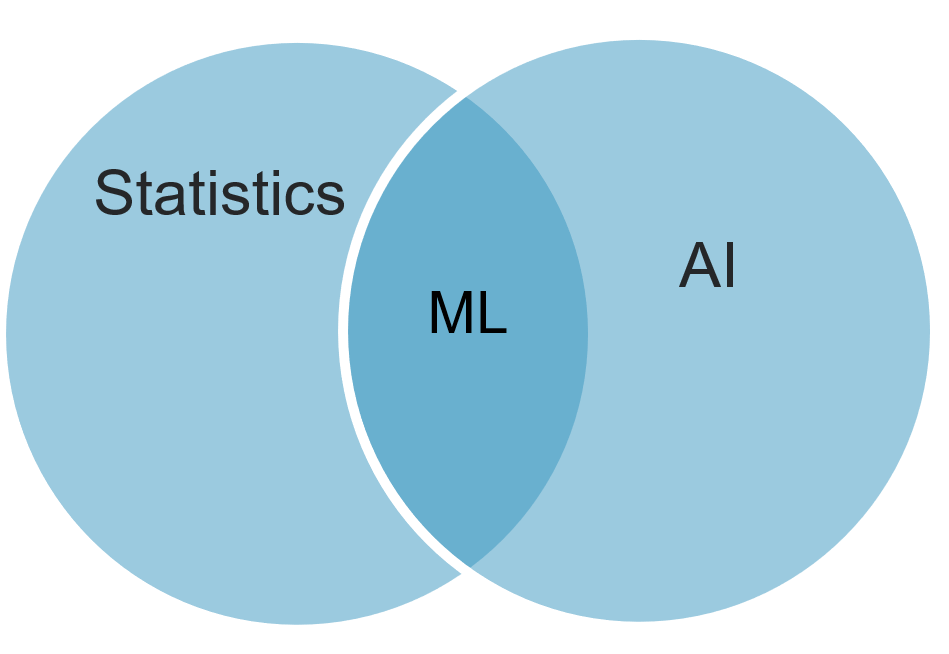
\includegraphics[width=0.6\textwidth]{pics/ml.png}
		\end{figure}
		
		\column{0.4\textwidth}
		\begin{block}{Focus on supervised ML}
			\begin{itemize}
				\item Regression
				\item Classification
			\end{itemize}
		\end{block}
		
		\begin{block}{Chapters}
			\begin{itemize}
				\item[3.] Linear Models
				\item[4.] Model Selection and Validation
				\item[5.] Trees
				\item[6.] Neural Nets
			\end{itemize}
		\end{block}
	\end{columns}
\end{frame}

\begin{frame}
	\frametitle{Model Setup}
	Approximate property $T$ of \alert{response} $Y$ (often $T = \E$) by function $f$ of $p$-dim \alert{covariate} vector $\bX = (X^{(1)}, \dots, X^{(p)})$ with value $\bx = (x^{(1)}, \dots, x^{(p)})$, i.e.,
	$$
		T(Y\mid \bX = \bx) \approx f(\bx)
	$$
	\vspace{-1.5em}
	\begin{itemize}
		\item Abbreviate $T(Y\mid \bX = \bx) = T(Y\mid \bx)$
		\item Estimate $f$ by $\hat f$ from data by minimizing objective
		$$
		Q(f) = \sum_{i = 1}^n L(y_i, f(\bx_i)) + \lambda \Omega(f)
		$$
		\item $L$: loss function in line with $T$; $\lambda \Omega(f)$: optional penalty
		\item $\boldsymbol y = (y_1, \dots, y_n)^T$: observed values of $Y$
		\item $\boldsymbol{\hat y} = (\hat y_1, \dots, \hat y_n)^T$: predicted/fitted values $\hat y_i = \hat f(\bx_i)$
		\item $\bx_1, \dots, \bx_n$: $n$ feature vectors; $x_i^{(j)}$: $i$-th value of $X^{(j)}$; $\bx^{(j)}$: $n$ values of feature $X^{(j)}$
	\end{itemize}
\end{frame}

%=====================================================================
\subsection{Linear Regression}
%=====================================================================

\begin{frame}
	\frametitle{Linear Regression}
	\begin{itemize}
		\item Postulate model equation
		$$
		\E(Y \mid \bx) = f(\bx) = \beta_o + \beta_1 x^{(1)} + \dots + \beta_p x^{(p)}
		$$
		\item Interpretation of parameters $\beta_j$? Ceteris Paribus!
		\item Optimal $\hat \beta_j$? Minimize sum of squared errors/residuals
		$$
		\sum_{i = 1}^n (\underbrace{y_i - \hat y_i}_{\text{\alert{Residual}}})^2 
		$$
		\item Remember: $\hat y = \hat f(\bx)$ are \alert{predictions}
	\end{itemize}
	
	\vfill
	
	\begin{example}
		Simple linear regression: $\E(Y \mid x) = \alpha + \beta x$
	\end{example}
\end{frame}

\begin{frame}
	\frametitle{Aspects of Model Quality}
	\begin{columns}[onlytextwidth]
		\column{0.5\textwidth}
		\begin{block}{Predictive performance}
			\begin{itemize}
				\item $\text{\alert{MSE}} = \frac{1}{n}\sum_{i = 1}^n (y_i - \hat y_i)^2$
				\item Root-MSE (\alert{RMSE})
				\item Relative performance: $R^2 = 1 - \text{MSE}/\text{MSE}_0$
				\item $\text{MSE}_0 \rightarrow$ intercept-only model
			\end{itemize}
		\end{block}	
		
		\column{0.5\textwidth}
		\begin{block}{Validity of assumptions}
			\begin{itemize}
				\item Model equation is correct
				\item \alert{Normal} linear model
				$$
				Y = f(\bx) + \varepsilon \text{ with }
				\varepsilon \sim N(0, \sigma^2)
				$$
			\end{itemize}
		\end{block}
	\end{columns}
	
	\vfill
	
	\begin{exampleblock}{\centering Example}
	\end{exampleblock}
\end{frame}

\begin{frame}
	\frametitle{Typical Problems}
	\begin{figure}
		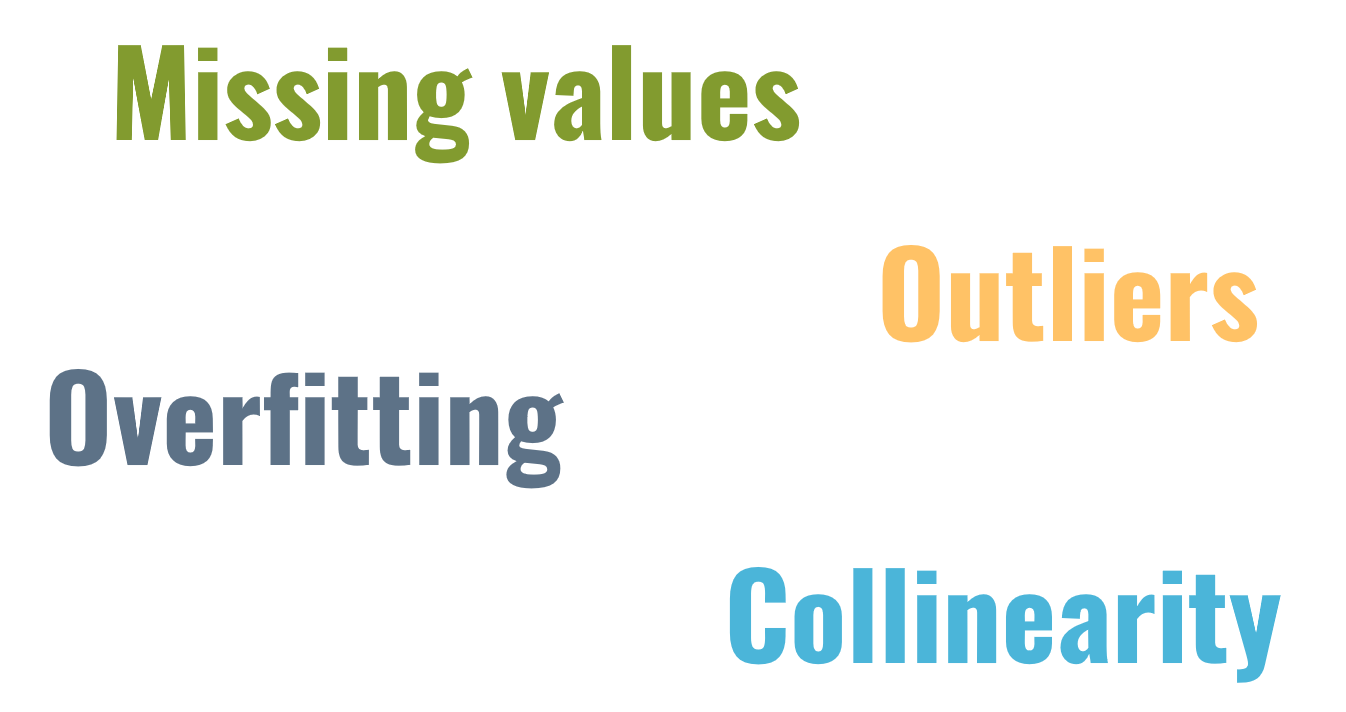
\includegraphics[width=0.7\textwidth]{pics/linear_problems.png}
	\end{figure}
\end{frame}

\begin{frame}
	\frametitle{Categorical Covariates}
	\begin{columns}[onlytextwidth]
		\column{0.45\textwidth}
		\begin{itemize}
			\item One-Hot-Encoding
			\item Dummy coding
			\item Interpretation?
		\end{itemize}
		
		\vspace{1cm}
		
		\begin{example}
		\end{example}
		
		\column{0.45\textwidth}
		\begin{block}{\centering Example of One-Hot-Encoding}
			\begin{small}
				\begin{table}
					\begin{tabular}{c|ccccccc}
						color& D& E& F &G&H &I &J \\
						\hline
						E  &   0  &   1  &   0  &   0  &   0  &   0  &   0 \\
						E  &   0  &   1  &   0  &   0  &   0  &   0  &   0 \\
						E  &   0  &   1  &   0  &   0  &   0  &   0  &   0 \\
						I  &   0  &   0  &   0  &   0  &   0  &   1  &   0 \\
						J  &   0  &   0  &   0  &   0  &   0  &   0  &   1 \\
						J  &   0  &   0  &   0  &   0  &   0  &   0  &   1 \\
						I  &   0  &   0  &   0  &   0  &   0  &   1  &   0 \\
						H  &   0  &   0  &   0  &   0  &   1  &   0  &   0 \\
						E  &   0  &   1  &   0  &   0  &   0  &   0  &   0 \\
						H  &   0  &   0  &   0  &   0  &   1  &   0  &   0 \\
						\hline
					\end{tabular}
				\end{table}
			\end{small}
		\end{block}
	\end{columns}
\end{frame}

\begin{frame}
	\frametitle{Linear Regression is Flexible}
	\begin{enumerate}
		\item Non-linear terms
		\item Interactions
		\item Transformations like logarithms
	\end{enumerate}
	
	\vfill
	
	\begin{alertblock}{These elements are essential but tricky!}
	\end{alertblock}
\end{frame}

\begin{frame}
	\frametitle{Non-Linear Terms}
	\begin{columns}
		\column{0.5\textwidth}
		\begin{block}{Deal with non-linear associations to $Y$?} $\rightarrow$ invest more parameters
			\begin{enumerate}
				\item Polynomial terms
				\begin{itemize}
					\item E.g., cubic regression
					$$
					\E(Y \mid x) = \beta_0 + \beta_1 x + \beta_2 x^2 + \beta_3 x^3
					$$
					\item Don't extrapolate!
				\end{itemize}
				\item Regression splines
			\end{enumerate}
		\end{block}
		
		\column{0.5\textwidth}
		\begin{block}{\centering Cubic terms for carat}
			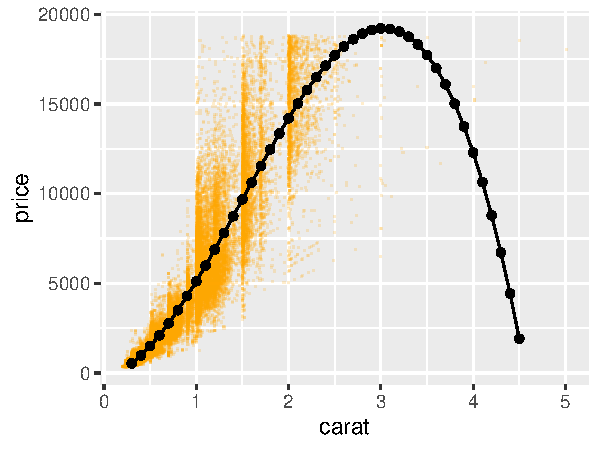
\includegraphics[width=1\textwidth]{pics/nonlinear.pdf}
			\vspace{-9em}
			\begin{scriptsize}
				\begin{table}
					\raggedleft
					\begin{tabular}{ccc}
						carat & carat$^2$ & carat$^3$ \\
						\hline
						0.23       &            0.0529       &          0.012167\\
						0.21       &            0.0441       &          0.009261\\
						0.23       &            0.0529       &          0.012167\\
						\hline
					\end{tabular}
				\end{table}
			\end{scriptsize}
			\vspace{3em}
			\centering Use systematic predictions
		\end{block}
	\end{columns}
\end{frame}

\begin{frame}
	\frametitle{Interactions}
	\begin{columns}
		\column{0.55\textwidth}
		\begin{itemize}
			\item Additivity of effects not always realistic
			$$
			\E(Y \mid \bx) = \beta_o + \beta_1 x^{(1)} + \dots + \beta_p x^{(p)}
			$$
			\item Adding interaction terms brings necessary flexibility 
			$\rightarrow$ more parameters
			\item Interaction between features $X$ and $Z$
			\begin{itemize}
				\item Multiplication (for categoricals?)
				\item For categorical $Z$, effects of $X$ are calculated by level of $Z$
				\item Like separate models per level of $Z$
			\end{itemize}
		\end{itemize}
		
		\column{0.45\textwidth}
		\begin{block}{\centering Carat and color}
			\begin{figure}
				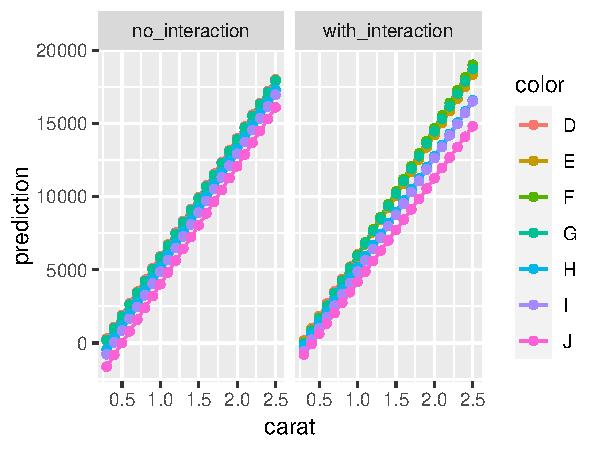
\includegraphics[width=\textwidth]{pics/interaction.pdf}
			\end{figure}
		\end{block}
	\end{columns}
\end{frame}

\begin{frame}
	\frametitle{Transformations of Covariates}
	\begin{block}{Examples}
		\begin{itemize}
			\item Dummy variables for categoricals
			\item Decorrelation
			\item Logarithms against outliers
		\end{itemize}
	\end{block}
	
	\vfill
	
	Effects are interpreted for transformed covariates
\end{frame}

\begin{frame}
	\frametitle{Logarithmic Covariates}
	\begin{itemize}
		\item $\E(Y \mid x) = \alpha + \beta\log(x)$
		\item Properties of logarithm allow interpretation \alert{for original covariate}
		\item A 1\% increase in $X$ is associated with an increase in $\E(Y)$ of about $\beta/100$
		\item Why?
		\begin{align*}
			\E(Y\mid 1.01x) - \E(Y\mid x) &= \alpha + \beta \log (1.01x) - \alpha - \beta \log(x) \\
			&= \beta \log\left(\frac{1.01x}{x}\right) \\
			&= \beta \log(1.01) \approx \beta/100
		\end{align*}
	
		\vfill
		
		\begin{example}
		\end{example}
	\end{itemize}
\end{frame}

\begin{frame}
	\frametitle{Logarithmic Responses}
	We see: log-transforming $X$ allows to talk about relative effects in $X$
	
	\vfill
	
	\begin{block}{Idea: log-transformed $Y$ allows to talk about relative effects on $Y$}
		Assume for a moment that
		$$
			\E(\log(Y) \mid x) = \alpha + \beta x \implies \log(\E(Y \mid x)) = \alpha + \beta x
		$$
		\vspace*{-1.2em}
		\begin{itemize}
			\item Multiplicative model $\E(Y\mid x) = e^{\alpha + \beta x}$
			\item Relative interpretation: ``A one-point increase in $X$ is associated with a relative increase in $\E(Y)$ of $100\%(e^\beta - 1)\approx 100\% \beta$''
			\item If also $\log(X)$?
		\end{itemize}
	\end{block}

	\vfill
	
	But assumption is wrong $\rightarrow$ biased predictions for $Y$ $\rightarrow$ GLMs

	\vfill
	
	\begin{exampleblock}{Examples}
	\end{exampleblock}
\end{frame}

\begin{frame}
	\frametitle{Example: Realistic Model for Diamond Prices}
	\begin{columns}
		\column{0.55\textwidth}
		\begin{itemize}
			\item Response: log(price)
			\item Covariates: log(carat), color, cut and clarity
		\end{itemize}
		
		\column{0.35\textwidth}
		\begin{figure}
			
\includegraphics[width=0.7\textwidth]{pics/dia2.png}
		\end{figure}
	\end{columns}
\end{frame}

%=====================================================================
\subsection{Generalized Linear Models}
%=====================================================================

\begin{frame}
	\frametitle{Generalized Linear Model (GLM)}
	\begin{block}{(One) extension of linear regression}
	\end{block}
	
	\begin{block}{Model equation}
		Two equivalent formulations
		\begin{align*}
			g(\E(Y \mid \bx)) &= \eta(\bx) = \beta_o + \beta_1 x^{(1)} + \dots + \beta_p x^{(p)} \\
			\E(Y \mid \bx) &=g^{-1}(\eta(\bx)) =  g^{-1}(\beta_o + \beta_1 x^{(1)} + \dots + \beta_p x^{(p)})
		\end{align*}
	\end{block}
	
	\begin{block}{Components}
		\begin{itemize}
			\item Linear function/predictor $\eta$
			\item Link function $g$ to map $\E(Y \mid \bx)$ to linear scale
			\item Distribution of $Y$ conditional on covariates $\rightarrow$ loss function (unit deviance)
		\end{itemize}
	\end{block}
\end{frame}

\begin{frame}
	\frametitle{Typical GLMs}
	\begin{columns}[onlytextwidth]
		\column{0.75\textwidth}
		\begin{figure}
			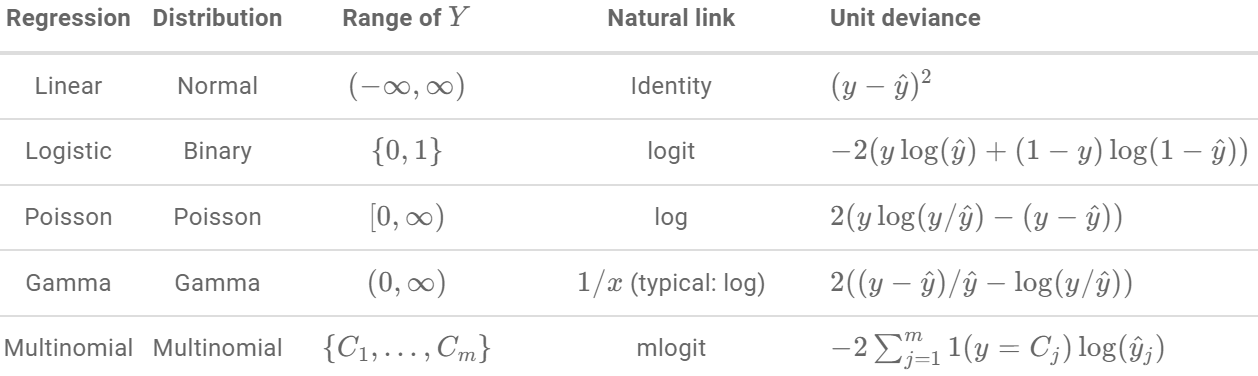
\includegraphics[width=1\textwidth]{pics/glm.png}
		\end{figure}
		\begin{figure}
			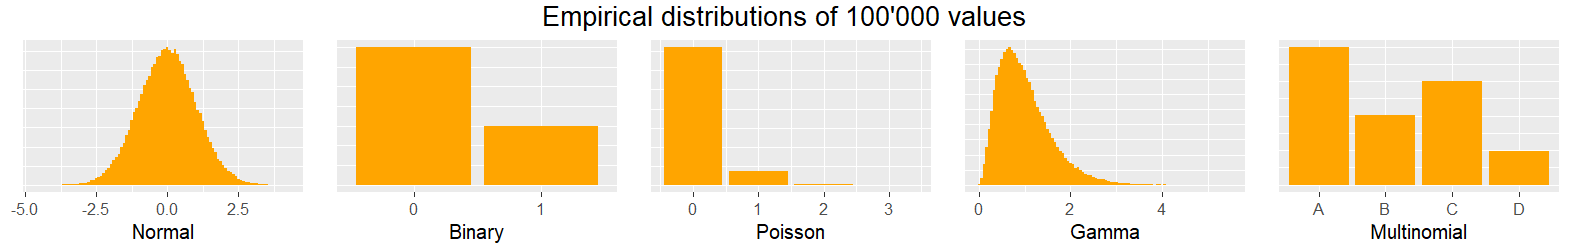
\includegraphics[width=1\textwidth]{pics/GLM_distributions.pdf}
		\end{figure}
		\column{0.25\textwidth}
		\begin{footnotesize}
			\begin{itemize}
				\itemsep0em 
				\item Predictions?
				\item Log-Link?
				\item For binary $Y$:
				$\E(Y) = P(Y = 1) = p$
				\item MSE $\rightarrow$ Deviance
				\item Losses in ML?
			\end{itemize}
		\end{footnotesize}
	\end{columns}
\end{frame}

\begin{frame}
	\frametitle{Why GLM, not Linear Regression?}
	\begin{block}{Linearity assumption not always realistic}
		\begin{enumerate}
			\item Binary $Y$: 
			
			Jump from 0.5 to 0.6 success probability less impressive than from 0.89 to 0.99
			\item Count $Y$: Jump from $\E(Y)$ of 2 to 3 less impressive than from 0.1 to 1.1.
			\item Right-skewed $Y$: 
			
			Jump from 1 Mio to 1.1 Mio deemed larger than from 2 Mio to 2.1 Mio.
		\end{enumerate}
		\alert{Logarithmic $Y$ not possible in the first two cases}
	\end{block}
	
	\vfill
	
	\begin{block}{GLM solves problem by suitable link $g$}
	\end{block}
	
	\vfill
	
	\begin{block}{Further advantages?}
	\end{block}
\end{frame}

\begin{frame}
	\frametitle{Interpretation of Effects guided by Link}
	\begin{columns}[onlytextwidth]
		\column{0.5\textwidth}
		\begin{block}{Identity link}
			Like linear regression
		\end{block}
		
		\begin{block}{Log link}
			Like linear regression with log response
			\begin{itemize}
				\item Multiplicative model for response
				\item Now in mathematically sound way
			\end{itemize}
		\end{block}
		
		\column{0.5\textwidth}
		\begin{block}{Logit link}
			\begin{itemize}
				\item Additive model for $\text{logit}(p)$
				\item $\text{logit}(p) = \text{\alert{log}}(\text{odds}(p)) = \text{\alert{log}}\left(\frac{p}{1-p}\right)$
				\item Remember: $p = P(Y=1) = \E(Y)$				
				\item Multiplicative model for $\text{odds}(p)$
				\item Coefficients \alert{$e^\beta - 1 \approx 100\%\beta$} interpreted as odds ratios
			\end{itemize}
		\end{block}
	\end{columns}
\end{frame}

\begin{frame}
	\frametitle{Examples with Insurance Claim Data}
	\begin{enumerate}
		\item Poisson regression for claim counts
		\item Binary logistic regression for claim (yes/no)
	\end{enumerate}
\end{frame}

%=====================================================================
\subsection{Modeling Large Data}
%=====================================================================

\begin{frame}
	\frametitle{Modeling Large Data}
	\begin{columns}[onlytextwidth]
		\column{0.55\textwidth}
		\begin{block}{As per 2023}
			\begin{itemize}
				\item On normal laptops, we can model datasets up to 8 GB in size
				(1 Mio iris data)
				\item Cloud computing allows 1000 times more
				\item We focus on in-memory situations
				
				$\rightarrow$ data fits in RAM
			\end{itemize}
		\end{block}
		
		\column{0.45\textwidth}
		\begin{block}{Aspect and example technology}
			\begin{enumerate}
				\item Data storage $\rightarrow$ Apache Parquet
				\item Data loading $\rightarrow$ Apache Arrow
				\item Preprocessing $\rightarrow$ data.table
				\item Modeling $\rightarrow$ H2O
			\end{enumerate}
			\vphantom{a}
		\end{block}
	\end{columns}

	\vfill
	
	\begin{example}
	\end{example}
\end{frame}
